\chapter{The master arm}
\label{ch:master}

The master is a miniature mannequin reproducing the Gen3's joint sequence at
roughly a third of its scale. The operator moves it with the fingers of one or
both hands. This chapter documents it completely: the mechanical chain, the
electronics, the firmware that turns fourteen analog channels and two inertial
sensors into a serial frame, and the signal conditioning applied on the way.
Source is at \repo{firmware/master\_arm/teensy\_final.ino}.

\section{Mechanical chain}

Each arm carries seven potentiometer-instrumented joints in an alternating
pattern: a roll about the preceding link's own axis, then a bend perpendicular
to it, repeated. \Cref{fig:kinchain} gives the sequence with the measured link
lengths, which sum to \SI{0.272}{\metre}.

The alternation is not incidental to the sensing design. A roll joint moves
the tip only through a downstream bend, because rotating a straight arm about
its own axis translates the tip by zero. A bend moves the tip directly. That
asymmetry is why the degradation ladder in \cref{ch:results} is ordered the
way it is, and why the loss of J2 or J4 costs reach while the loss of J3 or J5
costs almost nothing.

\begin{figure}[htbp]
  \centering
  % MASTER KINEMATIC CHAIN. Seven joints in an alternating roll/bend pattern,
% with the measured link lengths. Drawn straight (all joints at zero) so the
% lengths can be read off directly.
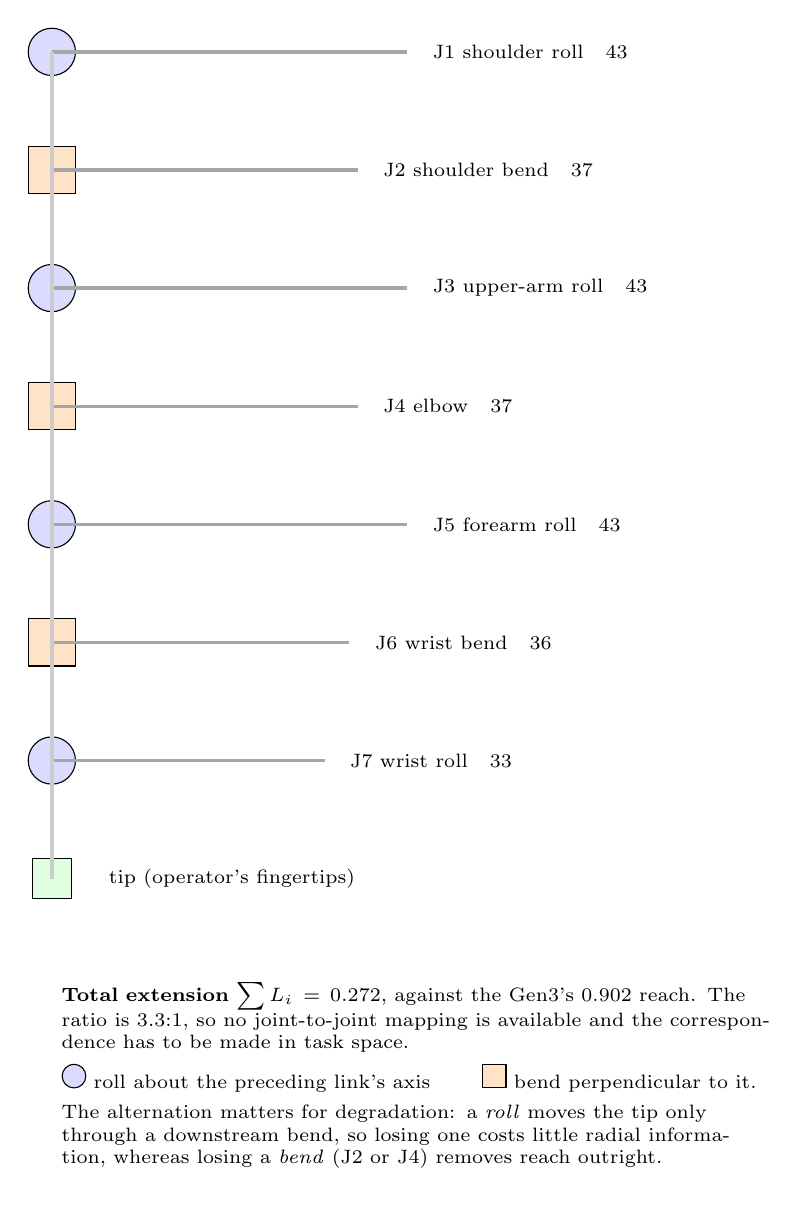
\begin{tikzpicture}[x=1mm, y=1mm, font=\scriptsize]

% The joint style is carried as a loop variable by NAME. Passing the style
% body directly fails: \foreach strips the braces and TikZ then reads the
% comma inside "circle, fill=blue!14" as an option separator, so "circle" is
% parsed as a colour.
\tikzset{
  jroll/.style = {draw, circle, fill=blue!14, minimum size=6mm, inner sep=0pt},
  jbend/.style = {draw, fill=orange!22, minimum size=6mm, inner sep=0pt},
}
\foreach \i/\len/\sty/\name in {
  1/43/jroll/{J1 shoulder roll},
  2/37/jbend/{J2 shoulder bend},
  3/43/jroll/{J3 upper-arm roll},
  4/37/jbend/{J4 elbow},
  5/43/jroll/{J5 forearm roll},
  6/36/jbend/{J6 wrist bend},
  7/33/jroll/{J7 wrist roll}}
{
  \pgfmathsetmacro{\y}{-\i*15}
  \pgfmathsetmacro{\w}{\len*1.05}
  \node[\sty] (j\i) at (0, \y) {};
  \draw[very thick, gray!70] (0,\y) -- (\w, \y);
  \node[anchor=west, font=\scriptsize] at (\w+2, \y)
     {\name \quad \SI{\len}{\milli\metre}};
}

\node[draw, fill=green!12, minimum size=5mm, inner sep=1pt] (tip) at (0, -120) {};
\node[anchor=west] at (6, -120) {tip (operator's fingertips)};

\draw[very thick, gray!40] (0,-15) -- (0,-120);

\node[anchor=north west, text width=90mm, align=left] at (0, -132)
  {\textbf{Total extension} $\sum L_i = \SI{0.272}{\metre}$, against the Gen3's
   \SI{0.902}{\metre} reach. The ratio is 3.3:1, so no joint-to-joint mapping
   is available and the correspondence has to be made in task space.\\[3pt]
   \tikz\node[draw, circle, fill=blue!14, minimum size=3mm, inner sep=0pt]{};\ %
   roll about the preceding link's axis \qquad
   \tikz\node[draw, fill=orange!22, minimum size=3mm, inner sep=0pt]{};\ %
   bend perpendicular to it.\\[3pt]
   The alternation matters for degradation: a \emph{roll} moves the tip only
   through a downstream bend, so losing one costs little radial information,
   whereas losing a \emph{bend} (J2 or J4) removes reach outright.};
\end{tikzpicture}

  \caption[Master kinematic chain]{The master's seven joints with measured
  link lengths, drawn at all joints zero so the lengths read off directly.}
  \label{fig:kinchain}
\end{figure}

\begin{figure}[htbp]
  \centering
  \imgplaceholder{55mm}{CAD render of one master arm, exploded, showing the
  seven potentiometer housings, the shaft couplings at each joint, the cable
  routing channel along each link, and the wrist platform carrying the
  MPU-6050 and the force-sensitive resistor. Must be dimensioned and must show
  how the cable bundle crosses each rotating joint, since that crossing is
  where the channel failures discussed in \cref{ch:results} originate.}
  \caption[Master arm CAD]{Master arm assembly. CAD render required before
  submission.}
  \label{fig:master-cad}
\end{figure}

\begin{figure}[htbp]
  \centering
  \imgplaceholder{55mm}{Photographs of the built master: (a) both arms on the
  shared shoulder frame, (b) close-up of one joint showing the potentiometer
  coupling, (c) the wrist platform with the IMU and FSR fitted, (d) the
  operator holding the master in the two-handed grip used in trials.}
  \caption[Master arm as built]{The assembled master. Build photographs
  required before submission.}
  \label{fig:master-photo}
\end{figure}

\section{Electronics}

A Teensy 4.1 reads every sensor and emits one text frame per cycle. The
sensor complement is fourteen rotary potentiometers, two MPU-6050 inertial
measurement units, two force-sensitive resistors and two momentary buttons.
\Cref{fig:electronics} gives the block diagram and the pin assignment;
\cref{tab:pinmap} gives the assignment in tabular form.

\begin{figure}[htbp]
  \centering
  % MASTER ARM ELECTRONICS. The pin assignment is the figure's real content,
% because the A4/A5 exclusion is what makes 16 analog channels sufficient.
\begin{tikzpicture}[x=1mm, y=1mm, font=\scriptsize]

\node[draw, thick, fill=gray!12, minimum width=44mm, minimum height=62mm,
      align=center] (mcu) at (0,0)
  {\textbf{Teensy 4.1}\\[2pt] i.MX RT1062\\ \SI{600}{\mega\hertz}\\[4pt]
   ADC \SI{12}{bit}\\ \texttt{analogReadAveraging(1)}\\[4pt]
   loop \SI{10}{\milli\second}\\ USB serial\\ \SI{115200}{baud}};

% ---- left: K1 pots
\node[draw, fill=blue!8, minimum width=30mm, align=center] (k1) at (-52, 20)
  {\textbf{K1 (left) pots}\\ 7 channels\\ \texttt{A0 A1 A2 A3}\\ \texttt{A6 A7 A8}};
\node[draw, fill=blue!8, minimum width=30mm, align=center] (k2) at (-52, 0)
  {\textbf{K2 (right) pots}\\ 7 channels\\ \texttt{A9 A10 A11}\\ \texttt{A12 A13 A16 A17}};
\node[draw, fill=blue!8, minimum width=30mm, align=center] (fsr) at (-52, -18)
  {\textbf{FSRs}\\ \texttt{A14} (left)\\ \texttt{A15} (right)};
\node[draw, fill=blue!8, minimum width=30mm, align=center] (btnn) at (-52, -34)
  {\textbf{buttons}\\ digital \texttt{2}, \texttt{3}\\ \texttt{INPUT\_PULLUP}};

% ---- right: I2C
\node[draw, fill=red!8, draw=red!60!black, thick, minimum width=32mm,
      align=center] (wire) at (52, 14)
  {\textbf{Wire (I\textsuperscript{2}C0)}\\ SDA pin 18 $=$ \texttt{A4}\\
   SCL pin 19 $=$ \texttt{A5}\\ \SI{400}{\kilo\hertz}};
\node[draw, fill=blue!8, minimum width=32mm, align=center] (imu1) at (52, -4)
  {\textbf{MPU-6050 \#1}\\ \texttt{0x68} (AD0 low)\\ left wrist};
\node[draw, fill=blue!8, minimum width=32mm, align=center] (imu2) at (52, -20)
  {\textbf{MPU-6050 \#2}\\ \texttt{0x69} (AD0 high)\\ right wrist};
\node[draw, fill=green!8, draw=green!45!black, minimum width=32mm,
      align=center] (host) at (52, -38)
  {\textbf{host}\\ \texttt{/dev/ttyACM*}\\ auto-detected};

\draw[flow] (k1.east)   -- (mcu.west |- k1.east);
\draw[flow] (k2.east)   -- (mcu.west |- k2.east);
\draw[flow] (fsr.east)  -- (mcu.west |- fsr.east);
\draw[flow] (btnn.east) -- (mcu.west |- btnn.east);
\draw[flow] (mcu.east |- wire.west) -- (wire.west);
\draw[thick] (wire.south) -- (imu1.north);
\draw[thick] (imu1.south) -- (imu2.north);
\draw[flow] (mcu.east |- host.west) -- (host.west);

% ---- the exclusion, called out
\node[draw, dashed, thick, red!60!black, fill=red!4, text width=74mm,
      align=left, font=\scriptsize] at (0, -50)
  {\textbf{\color{red!60!black}Why \texttt{A4} and \texttt{A5} carry no
   potentiometer.} The default \texttt{Wire} bus is pins 18/19, which
   \emph{are} \texttt{A4}/\texttt{A5}. An earlier revision listed both inside
   \texttt{potPinsK1}, so two pot channels shared conductors with the IMU data
   bus. Teensy~4.1 exposes 18 analog-capable pins; removing two leaves exactly
   16, which is what $14 + 2$ requires. \texttt{Wire1} (16/17) and
   \texttt{Wire2} (24/25) are never initialised, so \texttt{A2}, \texttt{A3},
   \texttt{A10} and \texttt{A11} are free as plain analog inputs.};

\end{tikzpicture}

  \caption[Master arm electronics]{Electronics architecture and pin
  assignment. The call-out explains why two analog-capable pins carry no
  potentiometer.}
  \label{fig:electronics}
\end{figure}

\begin{table}[htbp]
  \centering
  \caption{Pin assignment. Sixteen analog channels are required and sixteen
  are available once the two occupied by the default I\textsuperscript{2}C bus
  are excluded.}
  \label{tab:pinmap}
  \begin{tabular}{@{}llll@{}}
    \toprule
    Function & Count & Pins & Note \\
    \midrule
    K1 (left) potentiometers  & 7 & \texttt{A0 A1 A2 A3 A6 A7 A8} & no I\textsuperscript{2}C pins \\
    K2 (right) potentiometers & 7 & \texttt{A9 A10 A11 A12 A13 A16 A17} & no I\textsuperscript{2}C pins \\
    Force-sensitive resistors & 2 & \texttt{A14}, \texttt{A15} & left, right \\
    Buttons                   & 2 & digital \texttt{2}, \texttt{3} & \texttt{INPUT\_PULLUP} \\
    I\textsuperscript{2}C (\texttt{Wire}) & 2 & pin 18 $=$ \texttt{A4}, pin 19 $=$ \texttt{A5} & \textbf{excluded from analog use} \\
    \midrule
    \multicolumn{4}{@{}l@{}}{Analog-capable pins on Teensy 4.1: 18. Reserved
    for I\textsuperscript{2}C: 2. Remaining: \textbf{16}. Required: $14 + 2 =
    \mathbf{16}$.} \\
    \bottomrule
  \end{tabular}
\end{table}

\subsection{The A4 and A5 collision}

An earlier revision of the firmware listed \texttt{A4} and \texttt{A5} inside
the left arm's potentiometer array. Those two pins are not free. On the Teensy
4.1 the default \texttt{Wire} bus, which both inertial measurement units use,
is physically pins 18 and 19, and those pins \emph{are} \texttt{A4} and
\texttt{A5}. Two potentiometer channels were therefore sharing conductors with
the inertial sensors' data bus.

The failure mode this produces is not a clean one. Calling
\texttt{analogRead()} on a pin that the I\textsuperscript{2}C peripheral is
driving reconfigures that pin, so the effect appears as intermittent bus
corruption on the inertial sensors and as meaningless values on two
potentiometer channels, with the severity depending on the phase relationship
between the analog read and the bus transaction. Nothing about it looks like a
pin conflict from the outside.

The resolution was to exclude both pins from analog use entirely. The
arithmetic then works exactly: Teensy 4.1 exposes eighteen analog-capable
pins, removing two leaves sixteen, and sixteen is what fourteen potentiometers
plus two force sensors require. There is no spare, which is worth recording,
because any future channel needs either a multiplexer or a second board.

The two secondary I\textsuperscript{2}C buses are safe to use as plain analog
inputs and the design does so~\cite{pjrc2020teensy41}. \texttt{Wire1} occupies pins 16 and 17
(\texttt{A2}, \texttt{A3}) and \texttt{Wire2} occupies pins 24 and 25
(\texttt{A10}, \texttt{A11}), but neither peripheral is ever initialised: the
firmware calls only \texttt{Wire}. A bus that is never begun does not claim
its pins, so all four remain ordinary analog inputs and all four carry
potentiometers.

That headroom is the obvious route to a third and fourth inertial sensor. The
MPU-6050 family offers exactly two addresses, \texttt{0x68} and \texttt{0x69},
selected by the AD0 line, and both are already taken by the two wrist sensors.
A third sensor cannot join the same bus. Bringing up \texttt{Wire1} on pins 16
and 17 would carry another pair, at the cost of the two potentiometer channels
currently on \texttt{A2} and \texttt{A3}. \Cref{ch:results} quantifies why
that trade may be worth making.

\section{The inertial measurement driver}

The firmware includes a local \texttt{MPU6050.h} rather than an external
library. The reason is build portability: a sketch that depends only on
\texttt{Wire} compiles on any Arduino-compatible toolchain without a library
manager resolving versions, and the driver's behaviour is then fixed by the
source in the repository rather than by whatever version happens to be
installed.

\todo{CONFIRM: \repo{MPU6050.h} was not among the firmware files handed over
and is not in the repository. The interface below is the one the sketch calls
and is therefore certain; the register sequence is as specified by the author
and matches the device documentation, but the file itself should be attached
to the appendix before submission.}

Three entry points are used. \texttt{initialize()} wakes the device,
\texttt{testConnection()} confirms it is present and addressed correctly, and
\texttt{getMotion6()} returns six signed 16-bit values.

\paragraph{Waking the device.} The MPU-6050 powers up in sleep, with the
\texttt{SLEEP} bit of \texttt{PWR\_MGMT\_1} (register \texttt{0x6B}) set.
Until that bit is cleared the sensor registers read as
zero~\cite{invensense2013mpuregmap}. Clearing it is the whole of
initialisation for this application, since the power-on defaults for range and
filtering are the ones wanted.

\paragraph{Confirming presence.} \texttt{WHO\_AM\_I} (register \texttt{0x75})
returns a fixed identity value. Reading it distinguishes three states that
otherwise look identical from the outside: a sensor that is present and
responding, a sensor that is absent so the bus read returns nothing, and a
sensor that is present but strapped to the other address. The firmware prints
the verdict per sensor at start-up, and that line is the first thing to check
when one arm reports no orientation.

\paragraph{Reading the measurement.} All six axes plus temperature occupy
fourteen consecutive registers beginning at \texttt{ACCEL\_XOUT\_H}
(\texttt{0x3B}). The driver reads all fourteen in a single burst. This is not
only a bandwidth optimisation. The device latches its output registers for the
duration of a burst read, so a single transaction returns six axes from one
sampling instant, whereas six separate reads can straddle an internal update
and return a mixture of two. For an attitude estimate built from the ratio
between axes, a mixed sample is a wrong attitude rather than a noisy one.

Each axis arrives high byte first and is reassembled as a signed 16-bit value.
The two bytes of temperature sit between the accelerometer and gyroscope
blocks and are discarded here.

\subsection{Scale factors}

At the power-on defaults the accelerometer is at \(\pm\SI{2}{\gram}\) full
scale and the gyroscope at \(\pm\SI{250}{\degree\per\second}\), giving
sensitivities of \SI{16384}{LSB\per\gram} and
\SI{131}{LSB\per\degree\per\second}~\cite{invensense2013mpu6050}. The firmware
never changes the range registers, so these are the values that apply.

\begin{table}[htbp]
  \centering
  \caption{Inertial sensor scaling at power-on defaults.}
  \label{tab:imuscale}
  \begin{tabular}{@{}llll@{}}
    \toprule
    Quantity & Full scale & Sensitivity & Resolution \\
    \midrule
    Acceleration & $\pm\SI{2}{\gram}$ & \SI{16384}{LSB\per\gram}
      & \SI{61}{\micro\gram} per LSB \\
    Angular rate & $\pm\SI{250}{\degree\per\second}$
      & \SI{131}{LSB\per\degree\per\second}
      & \SI{7.6e-3}{\degree\per\second} per LSB \\
    \bottomrule
  \end{tabular}
\end{table}

A value of \SI{8192}{LSB\per\gram} is widely copied in example code and is
wrong for this configuration. It corresponds to the \(\pm\SI{4}{\gram}\)
range, which the device only enters if \texttt{ACCEL\_CONFIG} is written. Used
against the default range it halves every reported acceleration. That error
does not announce itself in the elevation estimate, because elevation is
computed from the direction of the acceleration vector and a uniform scale
error cancels in a normalised vector. It announces itself in the accelerometer
gate, which compares the vector's magnitude against \SI{1}{\gram} to decide
whether the sensor is measuring gravity alone: with the wrong scale, a
stationary sensor reports \SI{0.5}{\gram} and the gate rejects every frame.
The failure appears as a master that never produces a valid orientation, which
looks like a dead sensor.

\section{Signal conditioning}

\subsection{Potentiometers}

Each channel is read at 12-bit resolution with hardware averaging disabled,
then passed through an exponential moving average implemented in integer
arithmetic:

\begin{equation}
  e_{n+1} = \frac{\alpha\, r_n + (256 - \alpha)\, e_n}{256},
  \qquad \alpha = 64,
  \label{eq:ema}
\end{equation}

which is a smoothing factor of \num{0.25} per sample, realised as a shift
rather than a division. Integer arithmetic was chosen because the loop runs at
\SI{100}{\hertz} across sixteen channels and the Teensy's floating-point unit
is not needed for a filter whose input is a 12-bit integer.

The filtered count maps to degrees by a clamped linear transform:

\begin{equation}
  \theta = \SI{360}{\degree} \cdot
  \mathrm{clamp}\!\left(\frac{a - 50}{4045 - 50},\; 0,\; 1\right).
  \label{eq:adc2deg}
\end{equation}

The clamp limits are the substantive part. A potentiometer wiper never reaches
the extreme of its track, and the ends of the ADC range are where the reading
is least linear, so the transform discards the outer \num{50} counts at the
bottom and \num{50} at the top. The remaining \num{3995} counts span
\SI{360}{\degree}, giving \SI{0.090}{\degree} per count.

\subsection{A start-up transient in the filter initialisation}

\Cref{eq:ema} operates in raw ADC units: the steady state of the recurrence
for a constant input $r$ is $e = r$. The initialisation in \texttt{setup()}
does not match. It seeds each accumulator with \texttt{analogRead(pin) << 8},
which is \num{256} times the raw reading, a value consistent with a
fixed-point formulation the filter does not use.

Simulating the recurrence from that seed gives the transient in
\cref{tab:transient}. Every channel reads a railed \SI{360}{\degree} for
roughly the first \SI{190}{\milli\second} after reset and takes
\SI{440}{\milli\second} to settle.

\begin{table}[htbp]
  \centering
  \caption{Filter output after reset, simulated from \cref{eq:ema} with a
  constant input of \num{2000} counts and the seed used in \texttt{setup()}.}
  \label{tab:transient}
  \begin{tabular}{@{}rrr@{}}
    \toprule
    Cycle & Accumulator & Reported angle \\
    \midrule
     1 & \num{384500} & \SI{360.0}{\degree} (railed) \\
    10 & \num{30719}  & \SI{360.0}{\degree} (railed) \\
    20 & \num{3616}   & \SI{321.3}{\degree} \\
    25 & \num{2382}   & \SI{210.1}{\degree} \\
    30 & \num{2090}   & \SI{183.8}{\degree} \\
    44 & \num{2000}   & \SI{180.0}{\degree} (settled) \\
    \bottomrule
  \end{tabular}
\end{table}

Two consequences follow, and the second is the one that has cost time. Any
calibration capture taken within half a second of a board reset records a
railed or settling value rather than a joint angle. And re-opening the serial
port resets the board, so a calibration script that opens the port and
immediately samples is guaranteed to capture the transient. This is the same
window in which the inertial sensors are also settling, and the effects are
indistinguishable at the ROS level: both appear as a channel reporting a
plausible but wrong constant.

The existing calibration procedure already requires a settled stream before
sampling (\cref{fig:calibration}), for reasons that were diagnosed from the
gyroscope alone. The analysis here shows the potentiometers need the same
protection for a different reason. Correcting the seed to
\texttt{analogRead(pin)} removes the transient entirely and changes nothing
else, since the steady-state behaviour of \cref{eq:ema} is unaffected.
\todo{MEASURE: confirm the corrected seed on hardware and re-time the settling
window. The simulation above is arithmetic on the shipped recurrence, not a
measurement of the board.}

\subsection{A candidate explanation for the observed update rate}

The frame is emitted at \SI{100}{\hertz}, but recorded captures show each
potentiometer producing a new \emph{distinct} value at only
\SIrange{14.7}{17}{\hertz}, so \SIrange{82}{88}{\percent} of consecutive rows
repeat. That aliasing invalidated every per-row statistic computed before it
was noticed (\cref{ch:results}).

The firmware offers a mechanism. Angles are printed with one decimal place,
and \SI{0.1}{\degree} is \num{1.11} ADC counts. A smoothing factor of
\num{0.25} moves the filter only a quarter of the way to a new input in one
cycle, so a slow joint motion produces sub-count filter steps and the printed
value changes only when the accumulated motion crosses a printing boundary.
The effect is quantisation in the output format compounded with the filter,
not a slow sensor.

\todo{MEASURE: this explanation is consistent with the firmware but has not
been isolated. It is directly testable with \repo{scripts/virtual\_teensy.py},
which streams frames in the same wire format with known ground truth: sweep a
channel at a known rate and count distinct printed values against the
predicted boundary crossings. If confirmed, printing two decimals or raising
$\alpha$ recovers the full rate.}

\subsection{Force-sensitive resistors}

Both force sensors are read on the same 12-bit ADC as the potentiometers and
transmitted as integers. Measured pad values are \SIrange{6}{191}{counts}
unsqueezed and \num{3603} (left) and \num{3842} (right) at full squeeze, with
cross-talk of \SI{3.7}{\percent} and \SI{0.4}{\percent} under load only, so no
mixing matrix is required.

\todo{CONFIRM: the intended design applies a floating-point exponential
average to the force channels, so they carry decimal precision rather than
integer counts, and the ROS-side parser accepts a decimal in both force
fields. The firmware handed over transmits \texttt{\%d} and applies no filter
to these two channels. Either the float version was not the one delivered or
the change was not made; this should be resolved before the appendix listing
is fixed. The gripper mapping in \cref{ch:method} does not depend on it, since
it applies its own deadband and hysteresis downstream.}

\subsection{Buttons}

Both buttons are wired as two-wire switches to ground with
\texttt{INPUT\_PULLUP}, so the pin reads high when open and low when pressed
and no external resistor is needed. The firmware converts each press into a
latching toggle: a transition is accepted only if the raw level differs from
the last accepted level and at least \SI{40}{\milli\second} have passed since
the last accepted transition, and the output state flips only on the falling
edge.

Debouncing at the source matters more here than it usually would, because the
button is the clutch. A bounce that registers as two transitions toggles the
clutch twice, which disengages and re-engages it within a few milliseconds and
re-latches the anchor at whatever pose the master happened to be in. The
downstream clutch logic adds its own debounce and a quasi-static gate for the
same reason.

\section{The serial frame}

One frame is emitted per cycle, at \SI{100}{\hertz}, as ASCII text terminated
by a newline. \Cref{tab:frame} gives the fields in order. The format is
deliberately human-readable: a frame can be read directly from a terminal to
tell a wiring fault from a firmware fault without any host software running.

\begin{table}[htbp]
  \centering
  \caption{Serial frame, in transmission order. Fields are comma-separated;
  the frame ends with a newline. Buffer is \num{460} bytes against a typical
  frame of roughly \num{285}.}
  \label{tab:frame}
  \begin{tabular}{@{}llll@{}}
    \toprule
    Field & Count & Format & Meaning \\
    \midrule
    \texttt{k1j1}\ldots\texttt{k1j7} & 7 & \texttt{\%.1f}
      & left arm joint angles, \SIrange{0}{360}{\degree} \\
    \texttt{k2j1}\ldots\texttt{k2j7} & 7 & \texttt{\%.1f}
      & right arm joint angles, \SIrange{0}{360}{\degree} \\
    \texttt{K1IMU} & 6 & \texttt{\%d} $\times$ 6
      & left $a_x a_y a_z g_x g_y g_z$, raw LSB \\
    \texttt{K2IMU} & 6 & \texttt{\%d} $\times$ 6
      & right, same order \\
    \texttt{fsr1}, \texttt{fsr2} & 2 & \texttt{\%d}
      & grip force, raw counts \\
    \texttt{btn1}, \texttt{btn2} & 2 & \texttt{\%d}
      & latched toggle state, \num{0} or \num{1} \\
    \bottomrule
  \end{tabular}
\end{table}

Three properties of this format are relied on downstream. Inertial values are
transmitted \emph{raw}, in LSB, so the scale factors are applied on the host
and can be corrected without reflashing. The token \texttt{k1j1} at the start
of every frame is what the host's port auto-detection sniffs for, which is how
the board is found when it moves between \texttt{/dev/ttyACM0} and
\texttt{/dev/ttyACM1} across re-attachments. And the buttons carry a latched
state rather than an instantaneous level, so a host that misses frames cannot
miss a press.


\section{The CAD is not the kinematic source}
\label{sec:cad-not-kinematic}

This section exists so that nobody later mistakes the mechanical drawings for
the model the software uses. Three statements, each checked rather than
assumed.

\paragraph{The CAD carries no articulated joints.} Both STEP files declare the
\texttt{AUTOMOTIVE\_DESIGN} (AP214) schema, which \emph{is} capable of
carrying kinematic structure. Searching them for every entity that would
express it, \texttt{KINEMATIC\_JOINT}, \texttt{REVOLUTE\_PAIR},
\texttt{PRISMATIC\_PAIR}, \texttt{KINEMATIC\_LINK} and \texttt{MECHANISM},
returns zero occurrences in either file. They are solid geometry for
manufacture, drawn for three-dimensional printing, and they describe one fixed
configuration.

\paragraph{No robot description derives from them.} No URDF or xacro anywhere
in the workspace references \repo{PotArm.step}, \repo{backpack.step}, or any
\texttt{.step} file. More strongly: \textbf{the master arm has no URDF at
all.} It is not modelled as a robot description in any form.

\paragraph{The kinematics are seven measured constants.} What the software
actually uses is a single line,
\repo{srl\_teleop/master\_calibration.py}:

\begin{lstlisting}[language=Python]
LINK_LENGTHS = [0.043, 0.037, 0.043, 0.037, 0.043, 0.036, 0.033]
\end{lstlisting}

Those values did not come from the CAD. They originate in
\repo{basic\_control/kinematics.h} from the prior work
(\cref{ch:development}), where they are declared as ``physical link lengths
(metres), shaft-center to shaft-center, measured directly on the physical
master arm''. The chain is measured, not designed.

\paragraph{Why this matters, and why the agreement does not change it.}
\Cref{ch:results} reports that the CAD's joint-module pitch agrees with the
forward-kinematic link lengths to \SI{1.2}{\percent}. That is a genuine
cross-check and it is worth having, because until it was made those seven
numbers had never been compared against anything. It is emphatically
\textbf{not} a licence to treat the CAD as the source: the agreement was
established by measuring the CAD \emph{against} the constants, and the
constants remain the definition. If the two are ever found to disagree, the
question of which is correct is open and must be settled on the physical arm,
not by preferring whichever artefact is more convenient.

A successor tempted to regenerate the kinematics from the CAD should note that
it cannot be done: the geometry gives centre-to-centre pitch for a
\emph{pair} of joints and does not distinguish the \SI{43}{\milli\metre} roll
from the \SI{37}{\milli\metre} bend within it.

\section{Summary}

The master supplies fourteen joint angles, two three-axis accelerations, two
three-axis angular rates, two grip forces and two latched buttons, at
\SI{100}{\hertz} over USB serial. Of that, the position pipeline in
\cref{ch:method} consumes three or four potentiometer channels per arm and one
acceleration vector. The remainder is either used for orientation, used for
the gripper and clutch, or held in reserve against the loss of a channel that
is being used.
